\documentclass[journal,12pt,onecolumn]{IEEEtran}
\usepackage{cite}
\usepackage{amsmath,amssymb,amsfonts,amsthm}
\usepackage{algorithmic}
\usepackage{graphicx}
\usepackage{textcomp}
\usepackage{xcolor}
\usepackage{txfonts}
\usepackage{listings}
\usepackage{enumitem}
\usepackage{mathtools}
\usepackage{gensymb}
\usepackage{comment}
\usepackage[breaklinks=true]{hyperref}
\usepackage{tkz-euclide} 
\usepackage{listings}
\usepackage{gvv}      
\usepackage[latin1]{inputenc}                                
\usepackage{color}                                            
\usepackage{array}                                            
\usepackage{longtable}                                       
\usepackage{calc}                                             
\usepackage{multirow}    
\usepackage{hhline}                                           
\usepackage{ifthen}     
\usepackage{lscape}
\usepackage{tabularx}
\usepackage{array}
\usepackage{float}
\usepackage{multicol}
\usepackage{tikz}
\usepackage{pgfplots}
\pgfplotsset{compat=1.18} % or

\newtheorem{theorem}{Theorem}[section]
\newtheorem{problem}{Problem}
\newtheorem{proposition}{Proposition}[section]
\newtheorem{lemma}{Lemma}[section]
\newtheorem{corollary}[theorem]{Corollary}
\newtheorem{example}{Example}[section]
\newtheorem{definition}[problem]{Definition}
\newcommand{\BEQA}{\begin{eqnarray}}
\newcommand{\EEQA}{\end{eqnarray}}
\newcommand{\define}{\stackrel{\triangle}{=}}
\theoremstyle{remark}
\newtheorem{rem}{Remark}

\begin{document}
\bibliographystyle{IEEEtran}

\title{CE : GATE 2014}
\author{ai24btech11014 \\ Charitha Sri}
\maketitle

\section{SET-1}

\begin{enumerate}
    \item An isolated three-phase traffic signal is designed by Webster's method. The critical flow ratio for three phases are $0.20, 0.30,$ and $0.25$ respectively, and lost time per phase is 4 seconds. The optimum cycle length (in seconds) is \underline{\hspace{1cm}}.
 
    \item A levelling is carried out to establish the Reduced Levels (RL) of point R with respect to the Bench Mark (BM) at P. The staff readings taken are given below. \\
   \begin{table}[h]
        \centering
        \begin{tabular}{|c|c|c|c|c|}
        \hline
        Staff Station & BS & IS & FS & RL \\
        \hline
        P & 1.655m &  &  & 100.000m \\
        \hline
        Q & -0.950m &  & -1.500m & \\
        \hline
        R &  &  & 0.750m & ? \\
        \hline
        \end{tabular}
    \end{table}


    If RL of P is +100.000m, then RL (in m) of R is:
    \begin{enumerate}
        \begin{multicols}{2}
            \item $103.355$
            \item $103.155$
            \item $101.455$
            \item $100.355$
        \end{multicols}
    \end{enumerate}

    \item Group I lists tools/instruments, while Group II lists the corresponding surveying methods. Match the tool/instrument with the corresponding method of surveying.
     \begin{table}[h]
        \centering
        \begin{tabular}{|c|c|c|c|c|}
        \hline
        Staff Station & BS & IS & FS & RL \\
        \hline
        P & 1.655m &  &  & 100.000m \\
        \hline
        Q & -0.950m &  & -1.500m & \\
        \hline
        R &  &  & 0.750m & ? \\
        \hline
        \end{tabular}
    \end{table}


    \begin{enumerate}
        \begin{multicols}{2}
            \item P-3; Q-2; R-1; S-4
            \item P-2; Q-4; R-3; S-1
            \item P-1; Q-2; R-4; S-3
            \item P-3; Q-1; R-2; S-4
        \end{multicols}
    \end{enumerate}

\end{enumerate}
\section{SET-2}
\begin{enumerate}
    \item A fair (unbiased) coin was tossed four times in succession and resulted in the following outcomes: (i) Head, (ii) Head, (iii) Head, (iv) Head. The probability of obtaining a 'Tail' when the coin is tossed again is:
    \begin{enumerate}
        \begin{multicols}{4}
            \item $0$
            \item $\frac{1}{2}$
            \item $\frac{4}{5}$
            \item $\frac{1}{5}$
        \end{multicols}
    \end{enumerate}


\item The determinant of the matrix $\begin{pmatrix}
0 && 1 && 2 && 3 \\ 1 && 0 && 3 && 0 \\ 2 && 3 && 0 && 1 \\ 3 && 0 && 1 && 2 \end{pmatrix}$ is \underline{\hspace{1cm}}

\item $ z = \frac{2 - 3 i}{-5 + i}$ can be expressed as
\begin{enumerate}
    \begin{multicols}{2}
    \item $ -0.5 - 0.5i $
     \item $-0.5 + 0.5i$
      \item $0.5 - 0.5i$
       \item $0.5 + 0.5i$
    \end{multicols}
\end{enumerate}

\item The integrating factor for the differential equation $\frac{dP}{dt} + k_{2}P = k_{1}L_{0} e^{-k_{1}t}$ is 
\begin{enumerate}
\begin{multicols}{4}
    \item $e^{-k_{1}t}$
    \item $e^{-k_{2}t}$
     \item $e^{k_{1}t}$
    \item $e^{k_{2}t}$
\end{multicols}
\end{enumerate}

\item If $\brak{x}$ is a continuous, real valued random variable defined over the interval $\brak{-\infty, + \infty}$ and its occurence is defined by the density function given as: $f\brak{x} = \frac{1}{\sqrt{2 \pi}}b e^{\frac{-1}{2} {\brak{\frac{x - a}{b}}}^{2}}$ where $'a'$ and $'b'$ are the statistical attributes of the random variable $\brak{x}$. The value of the integral $\int_{-\infty}^{a} \frac{1}{\sqrt{2 \pi}}b e^{\frac{-1}{2} {\brak{\frac{x - a}{b}}}^{2}} dx$ is 

\begin{enumerate}
\begin{multicols}{4}
 \item $1$
 \item $0.5$
 \item $\pi$
 \item $\frac{\pi}{2}$
\end{multicols}
\end{enumerate}

\item Group I contains representative stress-strain curves as shown in the figure, while Group II gives the list of materials. Match the stress-strain  curves with the corresponding materials.


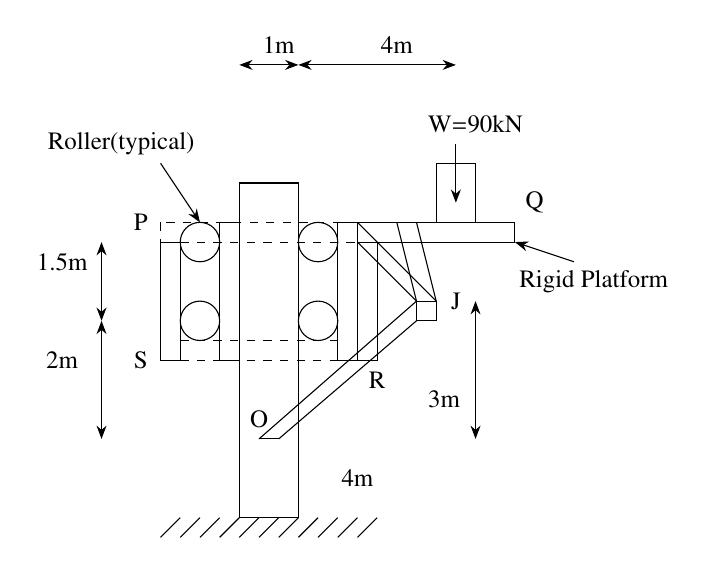
\begin{tikzpicture}
\tikzstyle{every node}=[font=\small]

% Draw rectangles
\draw (6.5,13.25) rectangle (7.25,9);
\draw (5.5,12.5) rectangle (5.75,11);
\draw (8,12.5) rectangle (8.25,11);
\draw (8,12.75) rectangle (10,12.5);
\draw (9,13.5) rectangle (9.5,12.75);
\draw (6.25,12.75) rectangle (6.5,11);
\draw (7.75,12.75) rectangle (8,11);
\draw (8.75,11.75) rectangle (9,11.5);

% Draw diagonal lines
\foreach \x in {5.75, 6, 6.25, 6.5, 6.75, 7, 7.25, 7.5, 7.75, 8, 8.25} {
    \draw (\x, 9) -- (\x - 0.25, 8.75);  % Diagonal lines going down left
}

% Draw additional diagonal lines connecting points at higher levels
\draw (8, 12.5) -- (8.75, 11.75);  % Diagonal line
\draw (8, 12.75) -- (9, 11.75);    % Diagonal line
\draw (8.5, 12.75) -- (8.75, 11.75); % Diagonal line
\draw (8.75, 12.75) -- (9, 11.75);  % Diagonal line


% Draw dashed lines
\draw [dashed] (8,12.75) -- (5.5,12.75);
\draw [dashed] (5.75,12.5) -- (8,12.5);
\draw [dashed] (5.5,12.75) -- (5.5,12.25);
\draw [dashed] (5.75,11.25) -- (7.75,11.25);
\draw [dashed] (5.75,11) -- (7.75,11);
\draw [<->, >=Stealth] (4.75,12.5) -- (4.75,11.5);
\draw [<->, >=Stealth] (4.75,11.5) -- (4.75,10);

% Draw circles
\foreach \y in {12.5, 11.5} {
    \draw (6, \y) circle (0.25cm);
    \draw (7.5, \y) circle (0.25cm);
}

% Draw lines for labels
\draw [-] (8.75,11.75) -- (6.75,10);
\draw [-] (8.75,11.5) -- (7,10);
\draw [-] (6.75,10) -- (7,10);

% Draw arrows
\draw [->, >=Stealth] (9.25,13.75) -- (9.25,13);
\draw [->, >=Stealth] (10.75,12.25) -- (10,12.5);
\draw [->, >=Stealth] (5.5,13.5) -- (6,12.75);
\draw [<->, >=Stealth] (6.5,14.75) -- (7.25,14.75);
\draw [<->, >=Stealth] (7.25,14.75) -- (9.25,14.75);
\draw [<->, >=Stealth] (9.5,11.75) -- (9.5,10);

% Add nodes
\node at (5.25,12.75) {P};
\node at (5.25,11) {S};
\node at (8.25,10.75) {R};
\node at (9.25,11.75) {J};
\node at (9.5,14) {W=90kN};
\node at (7,15) {1m};
\node at (8.5,15) {4m};
\node at (5,13.75) {Roller(typical)};
\node at (4.25,12.25) {1.5m};
\node at (6.75,10.25) {O};
\node at (8,9.5) {4m};
\node at (10.25,13) {Q};
\node at (11,12) {Rigid Platform};

\node at (9.1,10.5) {3m};
\node at (4.25,11.0) {2m};



\end{tikzpicture}


  \begin{table}[h]
        \centering
        \begin{tabular}{|c|c|c|c|c|}
        \hline
        Staff Station & BS & IS & FS & RL \\
        \hline
        P & 1.655m &  &  & 100.000m \\
        \hline
        Q & -0.950m &  & -1.500m & \\
        \hline
        R &  &  & 0.750m & ? \\
        \hline
        \end{tabular}
    \end{table}


    \begin{enumerate}
        \begin{multicols}{2}
            \item P-1; Q-3; R-2; 
            \item P-2; Q-3; R-1; 
            \item P-3; Q-1; R-2; 
            \item P-3; Q-2; R-1; 
        \end{multicols}
    \end{enumerate}

\item The first moment of area about the axis of bending for a beam cross-section is
   \begin{enumerate}
        \begin{multicols}{2}
        \item moment of inertia
        \item section modulus
        \item shape factor
        \item polar moment of inertia 
        \end{multicols}
    \end{enumerate}

    \item Polar moment of inertia $\brak{I_{P}}$ , in $cm^{4}$, of a rectangular section having width, $ b = 2 cm $ and depth $ d = 6 cm $  is \underline{\hspace{2cm}} 
    \item The target mean strength $f_{cm}$ for concrete mix design obtained from the charecteristic strength $f_{ck}$  and standard deviation $\sigma$, as defined in IS:456-2000, is
    \begin{enumerate}
        \begin{multicols}{2}
            \item $f_{ck} + 1.35 \sigma $
            \item $f_{ck} + 1.45 \sigma $
            \item $f_{ck} + 1.55 \sigma $
            \item $f_{ck} + 1.65 \sigma $
        \end{multicols}
    \end{enumerate}

\item The flexural tensile strength of M25 grade of concrete, in $N/mm^{2}$ as per IS:456-2000 is \underline{\hspace {1 cm}}


\end{enumerate}
\end{document}
